\documentclass{beamer}
\usetheme{CambridgeUS}
\usecolortheme{dolphin}
%themes to test
%Theme to: AnnArbor Antibes Bergen Berkeley Berlin Boadilla boxes CambridgeUS Copenhagen Darmstadt default Dresden Frankfurt Goettingen Hannover Ilmenau JuanLesPins Luebeck Madrid Malmoe Marburg Montpellier PaloAlto Pittsburgh Rochester Singapore Szeged Warsaw
%Color to: albatross beaver beetle crane default dolphin dove fly lily orchid rose seagull seahorse sidebartab structure whale wolverine
%Font to: default professionalfonts serif structurebold structureitalicserif structuresmallcapsserif

%allows picture file insertion into document
\usepackage{graphicx}

%sets numbered citation and uses bib.bib as bibliography file
\usepackage[natbib=true, style=numeric, sorting=none]{biblatex}
\renewcommand*{\bibfont}{\tiny}
\addbibresource{bib.bib}

%sets size of footnote citation to \tiny
\setbeamerfont{footnote}{size=\tiny}

\title{Hyperkalemia: Diagnosis and Treatment}
\author{Eric W. Robbins}
\date{Last updated: 11/01/2021}
\begin{document}
	\begin{frame}
		\maketitle
	\end{frame}
	\begin{frame}
		\frametitle{Table of Contents}
		\tableofcontents
	\end{frame}
\section{Overview}
\subsection{Why Care}
\begin{frame}
\frametitle{Why Care}
\centering
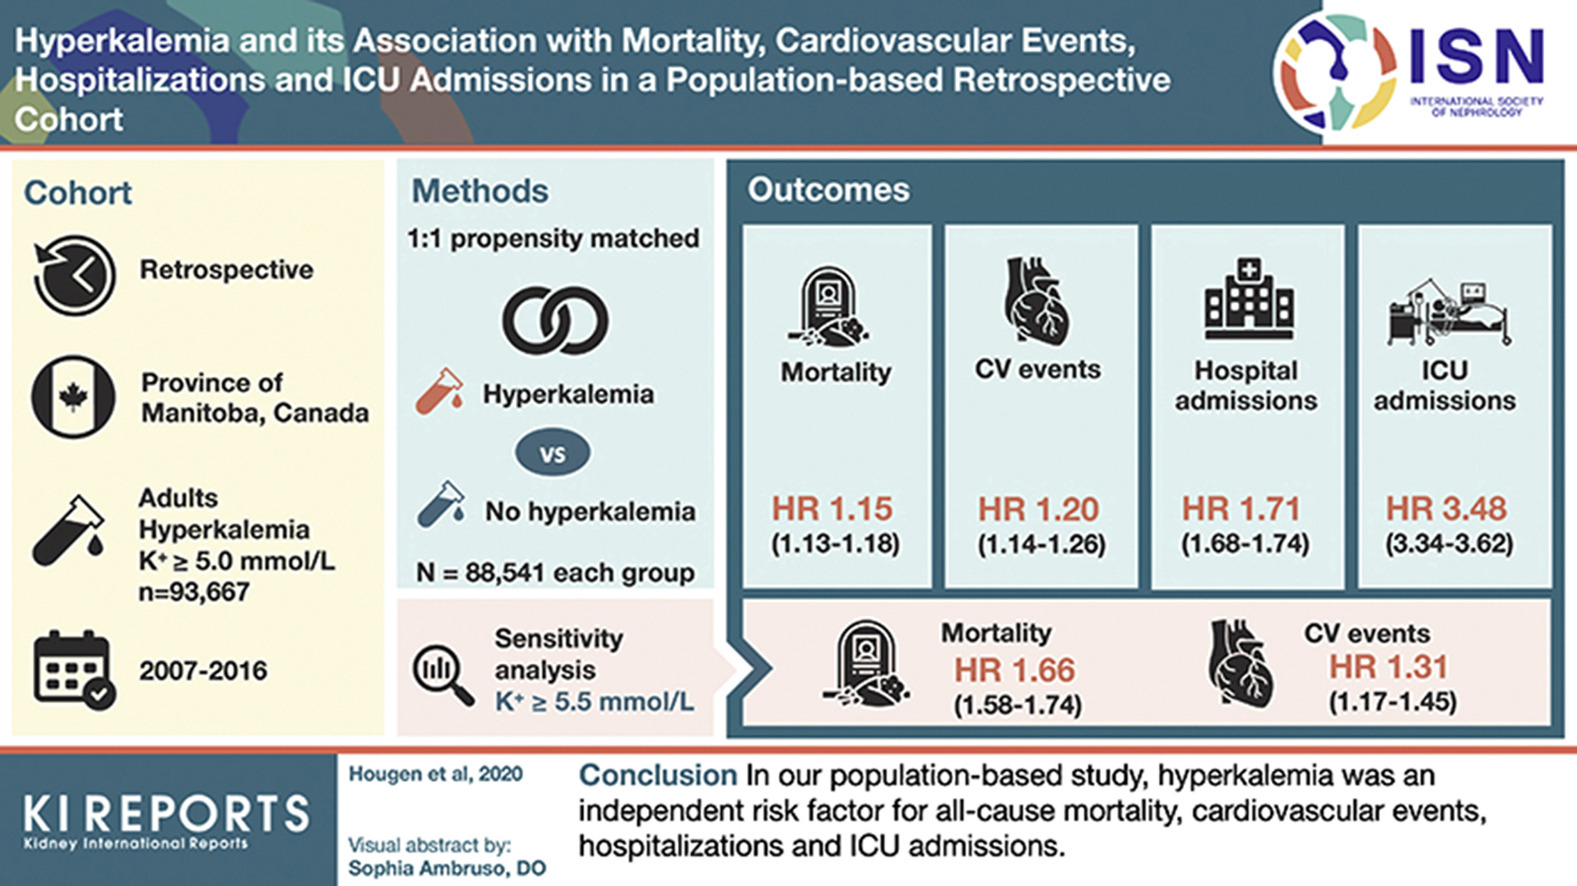
\includegraphics[width=0.90\textwidth,keepaspectratio]{media/danger.jpg}
\\
\tiny{Source:}
\footfullcite{Hougen2021}
\end{frame}
\subsection{When to Care}
	\begin{frame}
		\frametitle{When to Care}
		\begin{itemize}
			\item EKG changes
			\pause
				\begin{itemize}
					\item peaked T waves
					\item PR depression
					\item bradycardia (!)
					\item sinusoidal pattern (!!)
				\end{itemize}
			\pause
			\item How Useful is the EKG?
			\pause
				\begin{itemize}
					\item study of ESRD pts getting emergent HD (n = 317)\footfullcite{Rafique2020}
					\item SEN 0.19, SPEC 0.97, PPV 0.92, NPV 0.46
					\item Other studies were worse \footfullcite{Wrenn1991}
				\end{itemize}
			\pause
			\item What about Cardiologists?\footfullcite{Montague2008}
			\pause
			\begin{itemize}
				\item n = 90 of K $\geq$6.0
				\item n = 24 had ``T wave changes'' (21 were non-specific)
				\item n = 3 had ``Peaked T waves'' (3.33\%)
			\end{itemize}
		\end{itemize}
	\end{frame}
\subsection{Formal Definition}
\begin{frame}
\frametitle{Formal Definition}
	\centering
	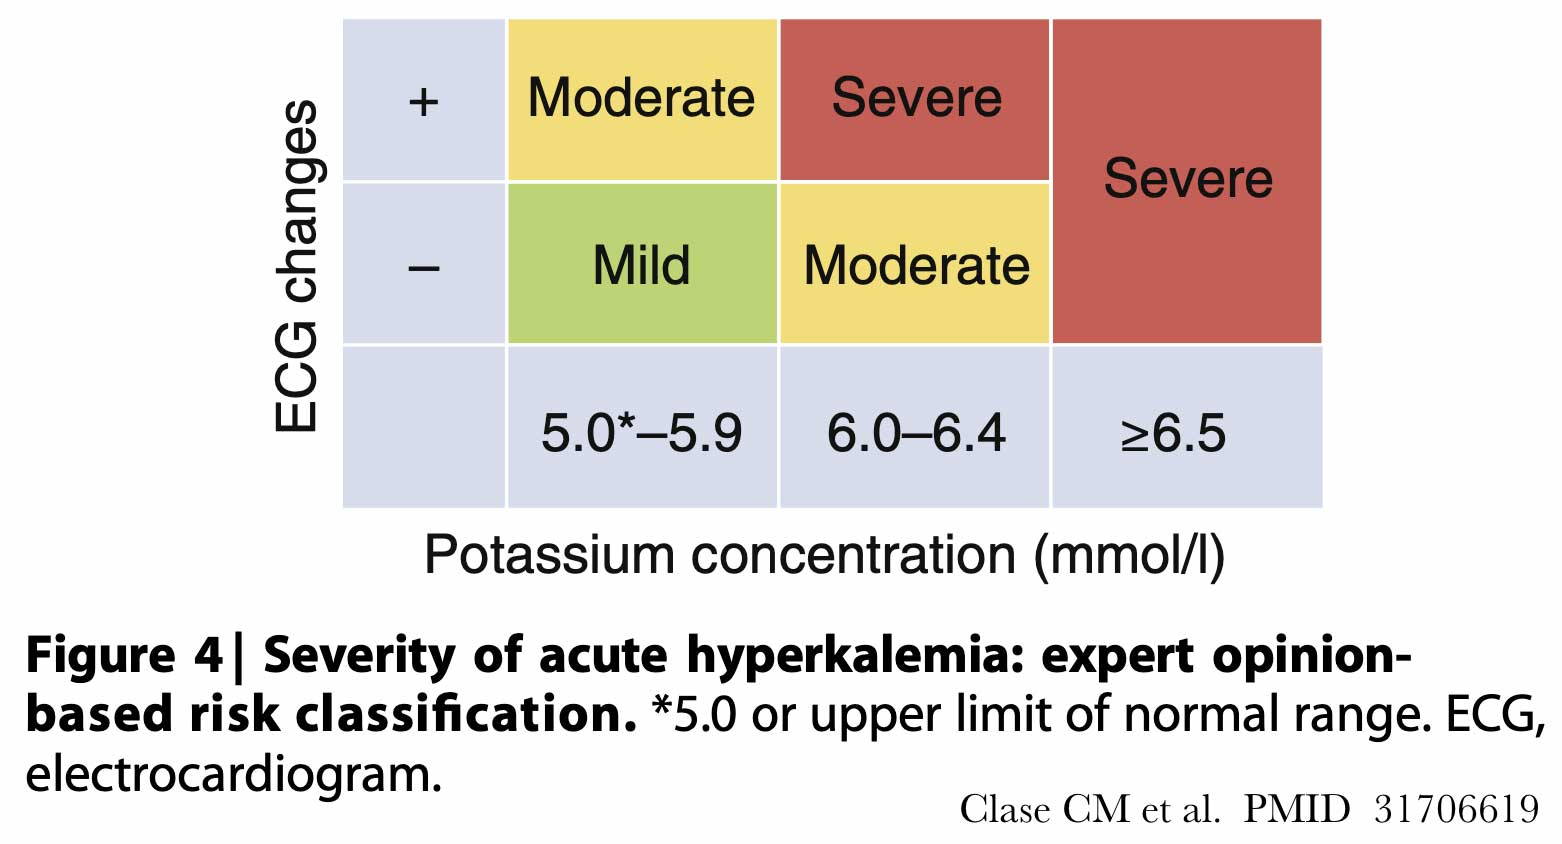
\includegraphics[width=0.90\textwidth,keepaspectratio]{media/definition.jpg}
	\\
	\tiny{Source:}\footfullcite{Clase2020}
\end{frame}
\section{Therapies}
\begin{frame}
	\frametitle{What Works}
		\begin{itemize}
			\item Myocardial Stabilization
			\item Push K Back In
			\item Get Rid of K
			\item Prevent Recurrence
		\end{itemize}
\end{frame}
\subsection{Myocardial Stabilization}
\begin{frame}
	\frametitle{Myocardial Stabilization}
	Clinical Pearls
		\begin{itemize}
			\item Saves lives!
			\item Gluconate vs Chloride
			\begin{itemize}
				\item 1\textendash 3 g CaGluc or 1 g CaCl\footfullcite{Clase2020}
				\end{itemize}
			\item Redosing?
			\begin{itemize}
				\item Optimal regimen unknown\footfullcite{LaRue2017}
				\item Calcium only lasts for 30\textendash60 min
				\item Redose if unstable arrhythmia (brady, wide QRS)
			\end{itemize}
		\end{itemize}
\end{frame}
\subsection{Pushing K Back In}
\begin{frame}
	\frametitle{Pushing K Back In}
	\begin{itemize}
		\item Options%XKd6!%U^5wY&wd4KSS9$0adJ@tKaF\left( 
		\pause
			\begin{itemize}
				\item \emph{IV} insulin $\pm$ dextrose
				\item $\beta$2 agonists
					\begin{itemize}
						\item albuterol data is old (1980s\textendash early 1990s)\footfullcite{Allon1989,Allon1990}
						\item or is on IV salbutamol\footfullcite{Liou1994,Mandelberg1999}
						\item for unstable bradycardia $\pm$ shock, use epinephrine drip
					\end{itemize}
				\item if no hypervolemia, isotonic bicarb (D5W with 150 mEq/L NaHCO3)
					\begin{itemize}
						\item per old RCTs, bicarb \emph{ampules} don't work
					\end{itemize}
			\end{itemize}
	\end{itemize}
\end{frame}
\subsection{Getting Rid of K}
\begin{frame}
	\frametitle{Getting Rid of K}
	\pause
			\begin{columns}
				\column{0.5\textwidth}
				\centering
				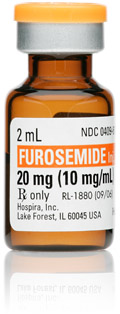
\includegraphics[height=.4\textheight,keepaspectratio]{media/lasix.png}
				\column{0.5\textwidth}
				\centering
				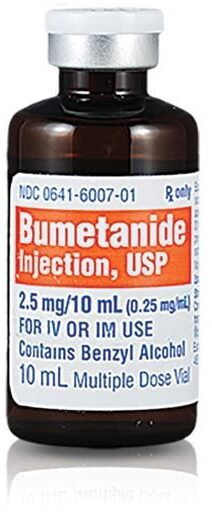
\includegraphics[height=.4\textheight,keepaspectratio]{media/bumex.jpeg}
			\end{columns}
			\begin{columns}
				\column{0.5\textwidth}
				\centering
				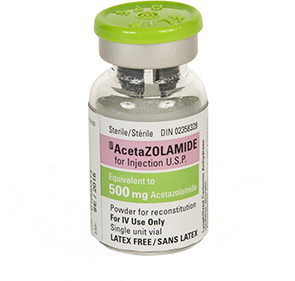
\includegraphics[height=.4\textheight,keepaspectratio]{media/acetazolamide.png}
				\column{0.5\textwidth}
				\centering
				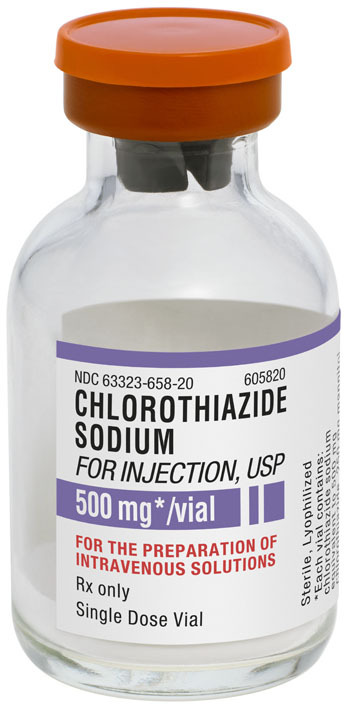
\includegraphics[height=.4\textheight,keepaspectratio]{media/chlorothiazide.jpg}
			\end{columns}
\end{frame}
\subsection{Preventing Recurrence}
\begin{frame}
	\frametitle{Preventing Recurrence}
	\pause
		\begin{columns}
			\column{0.5\textwidth}
			\centering
			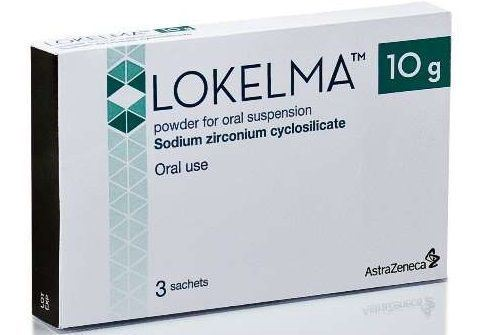
\includegraphics[width=.9\textwidth,keepaspectratio]{media/lokelma.jpg}
			\column{0.5\textwidth}
			\centering
			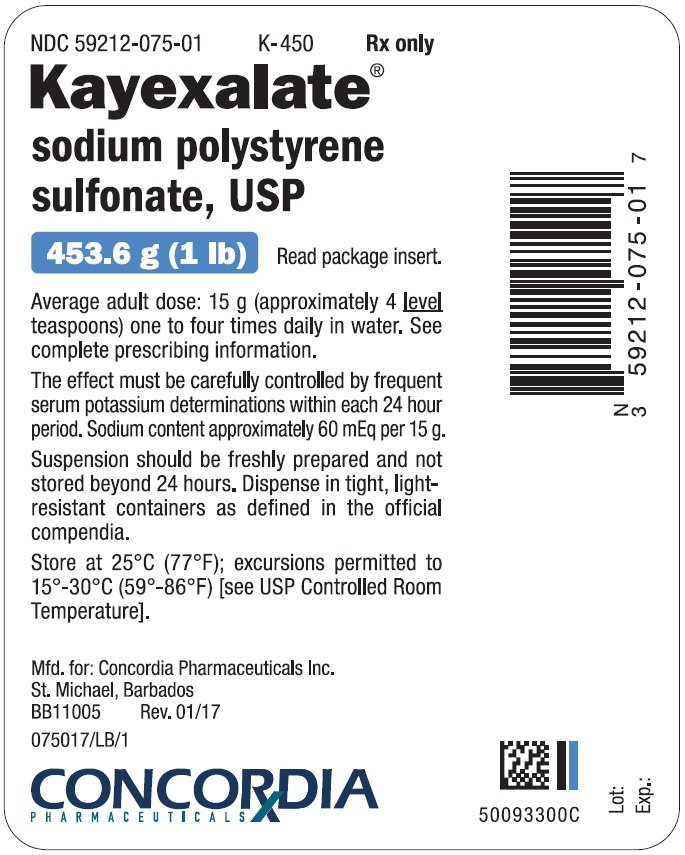
\includegraphics[width=.9\textwidth,keepaspectratio]{media/kayexalate.jpg}
		\end{columns}
\end{frame}
\section{Conclusions}
\begin{frame}
	\frametitle{Conclusions}
	\begin{itemize}
		\item Diagnose
		\begin{itemize}
			\item Don't use EKG to decrease your concern
		\end{itemize}
		\item Myocardium
		\begin{itemize}
			\item CaGluc or CaCl saves lives
		\end{itemize}
		\item Temporize
		\begin{itemize}
			\item IV insulin
			\item IV diuretics
			\item IV bicarb or LR
		\end{itemize}
		\item Reduce recurrence
		\begin{itemize}
			\item sodium zirconium cyclosilicate (Lokelma)
		\end{itemize}
	\end{itemize}
\end{frame}
\section{References}
\begin{frame}
	\frametitle{References}
	\printbibliography
\end{frame}
\end{document}
